\documentclass[11pt]{asaproc}\usepackage[]{graphicx}\usepackage[]{color}
%% maxwidth is the original width if it is less than linewidth
%% otherwise use linewidth (to make sure the graphics do not exceed the margin)
\makeatletter
\def\maxwidth{ %
  \ifdim\Gin@nat@width>\linewidth
    \linewidth
  \else
    \Gin@nat@width
  \fi
}
\makeatother

\definecolor{fgcolor}{rgb}{0.345, 0.345, 0.345}
\newcommand{\hlnum}[1]{\textcolor[rgb]{0.686,0.059,0.569}{#1}}%
\newcommand{\hlstr}[1]{\textcolor[rgb]{0.192,0.494,0.8}{#1}}%
\newcommand{\hlcom}[1]{\textcolor[rgb]{0.678,0.584,0.686}{\textit{#1}}}%
\newcommand{\hlopt}[1]{\textcolor[rgb]{0,0,0}{#1}}%
\newcommand{\hlstd}[1]{\textcolor[rgb]{0.345,0.345,0.345}{#1}}%
\newcommand{\hlkwa}[1]{\textcolor[rgb]{0.161,0.373,0.58}{\textbf{#1}}}%
\newcommand{\hlkwb}[1]{\textcolor[rgb]{0.69,0.353,0.396}{#1}}%
\newcommand{\hlkwc}[1]{\textcolor[rgb]{0.333,0.667,0.333}{#1}}%
\newcommand{\hlkwd}[1]{\textcolor[rgb]{0.737,0.353,0.396}{\textbf{#1}}}%
\let\hlipl\hlkwb

\usepackage{framed}
\makeatletter
\newenvironment{kframe}{%
 \def\at@end@of@kframe{}%
 \ifinner\ifhmode%
  \def\at@end@of@kframe{\end{minipage}}%
  \begin{minipage}{\columnwidth}%
 \fi\fi%
 \def\FrameCommand##1{\hskip\@totalleftmargin \hskip-\fboxsep
 \colorbox{shadecolor}{##1}\hskip-\fboxsep
     % There is no \\@totalrightmargin, so:
     \hskip-\linewidth \hskip-\@totalleftmargin \hskip\columnwidth}%
 \MakeFramed {\advance\hsize-\width
   \@totalleftmargin\z@ \linewidth\hsize
   \@setminipage}}%
 {\par\unskip\endMakeFramed%
 \at@end@of@kframe}
\makeatother

\definecolor{shadecolor}{rgb}{.97, .97, .97}
\definecolor{messagecolor}{rgb}{0, 0, 0}
\definecolor{warningcolor}{rgb}{1, 0, 1}
\definecolor{errorcolor}{rgb}{1, 0, 0}
\newenvironment{knitrout}{}{} % an empty environment to be redefined in TeX

\usepackage{alltt}
\usepackage{graphicx}
\usepackage{setspace}
\usepackage{amsmath}

\doublespacing

\title{An Analysis of the Impact of Rent Control on New York City Housing}
\author{Benjamin W. Schweitzer \and Thomas J. Fisher \and Karsten Maurer \and Alison Tuiyott \and Lydia Carter \and Robert Garrett}
\IfFileExists{upquote.sty}{\usepackage{upquote}}{}
\begin{document}

\maketitle

\begin{abstract}
It is the concern of policy makers every year in New York whether or not the enacted rent control policy has a positive effect on the New York City rental market. In order to measure the effectiveness of this policy, we aim to study the change of housing quality and the impact it had on the lives of people who live within these rent controlled homes. We create a housing quality index metric and study how it changes over time in relationship to rent-controlled versus non-rent controlled. The impact of rent control on housing and life quality will be assessed, thus assessing policy effectiveness.
\begin{keywords}
Rent Control, Survey Analysis, Multivariate Multiple Regression
\end{keywords}
\end{abstract}

\section{Introduction\label{intro}}

For the 2019 Statistical Computing Data Expo my fellow contestants and I were provided with New York City Housing and Vacancy Survey data from 1991 to 2017 along with a series of guided question that we could pursue for our research project. The topic that we decided upon addressing was related to rent control policy.

Rent control policy in New York is an extremely influential and complex system that effects millions of homes in New York City. Rent control policy has taken on many forms throughout the years and is subject to a great deal of debate criticism towards how it is being implemented and the effectiveness of proposed implementations. The goal of the research project was to introduce a way to model the effect of New York City rent control policy on the quality of housing in New York City over the last twenty years.

Using the surveys provided, we aggregated three measures of damage to describe the condition of a house (external, utility, and pest). We then modeled these damages with multiple predictor variables including an indicator of rent control in attempt to isolate and measure the effect of these predictor variables on the housing damages. Through interpretation of model coefficients, we were able to observe the modeled relationships between predicted damage rates 

\section{Data\label{data}}
\subsection{New York City Housing and Vacancy Survey}
The data provided for the competition was from the New York City Housing and Vacancy Survey from the years of 1991, 1993, and then every three years up until 2017. The data consists of over 130 features and 14000 rows of coded survey responses for one unit to a variety of questions that have a corresponding data dictionary for each year that allows you to decode the surveys. The questions give information about the physical conditions of the unit, various costs of living, demographic information about persons living in the unit, rent control information about the unit, persons living in the unit’s opinions on the unit, survey weights, and a vast amount of information about each unit surveyed. 
\subsection{Survey Aggregation}
We identified the variables that would indicate a physical external damage to the home such as a broken window, hole in the floor, cracked stairwell, etc. and aggregated across all these and if any damage was present our new indicator variable External Damage would have a value of 1, 0 if no damages are present. The same process was repeated for our indicators of Utility Damage and Pest Damage where we would aggregate across variable that indicate that corresponding damage. We also used this process to determine whether or not a unit was under rent control, since there are many variables that indicate whether or not a unit is under a specific kind of rent control policy so we were able to reduce this into one single feature that would indicate whether or not a unit was under some form of rent control policy. Lastly removed the homes that were above the 75th percentile of monthly rent costs since we deemed them to not be the target of rent control policy, and then binned the remaining units by quartiles and created a variable that indicated which monthly rent quartile a unit would be classified under.

Now each row represents a unit that has all of these varaibles we have created through aggregation, an identifier of year, an identifier of borough, and indentifier of sub-borough, and the survey weight applied to the unit. We then grouped units by year, rent control, rent quartile, borough, and sub-borough to get proportion of homes with eacch of the three types of damage for each group.
\subsection{Exploratory Data Analysis}
This data set can be explored visually to identify trend in the data that might be useful during the modeling stage. In figure 1, you can see the proportion of homes with an external damage partitioned by borough, rent quartile, and whether or not the home was under rent control. It is clear that in almost all bouroughs, for each rent quartile, the porporiton of rent controlled homes with an external damage is higher than than the proportion of homes not under rent control with an external damage. This trend is seen in most years in all three damage types, indicating there may a correaltion bewtween rent control status and higher damage rates.

In Figure 2, you can see the median sub-borough utility damage rate of homes in Brooklyn over time, along with bands that represent the middle 50 percent of sub-borough damage rates that were used to calculate the borough wide porportion. You can see that there exists a gap between the rent controlled and non rent controlled damage rates each year. This may reinforce the trend we started to see in figure 1, indicating we may see some positive correlation between rent control status and higher damage rates in the three categories.
 


\begin{figure}
\begin{center}
\begin{knitrout}
\definecolor{shadecolor}{rgb}{0.969, 0.969, 0.969}\color{fgcolor}
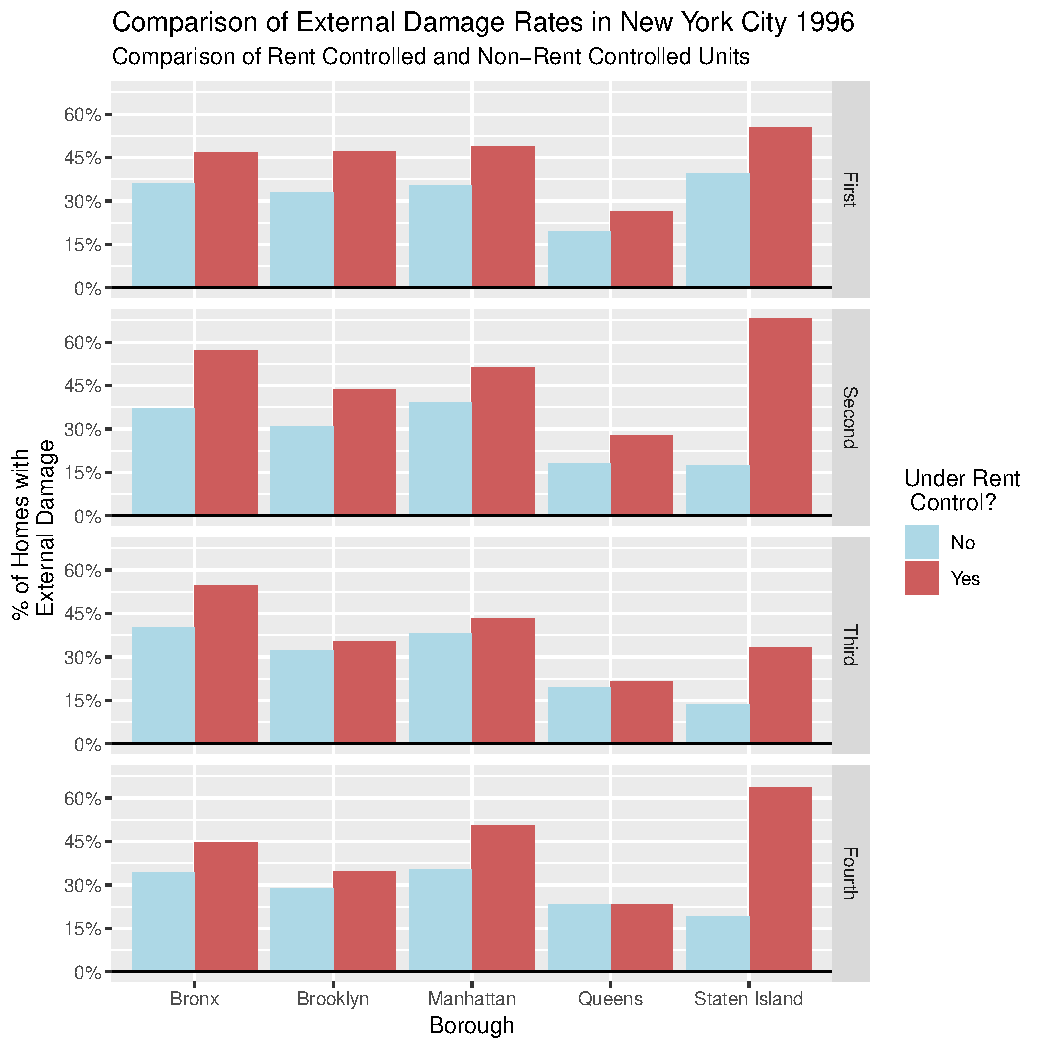
\includegraphics[width=\maxwidth]{figure/fig1-1} 

\end{knitrout}
\end{center}
\caption{External Damage Rate Plot}
\label{fig:one}
\end{figure}

\begin{figure}
\begin{center}
\begin{knitrout}
\definecolor{shadecolor}{rgb}{0.969, 0.969, 0.969}\color{fgcolor}
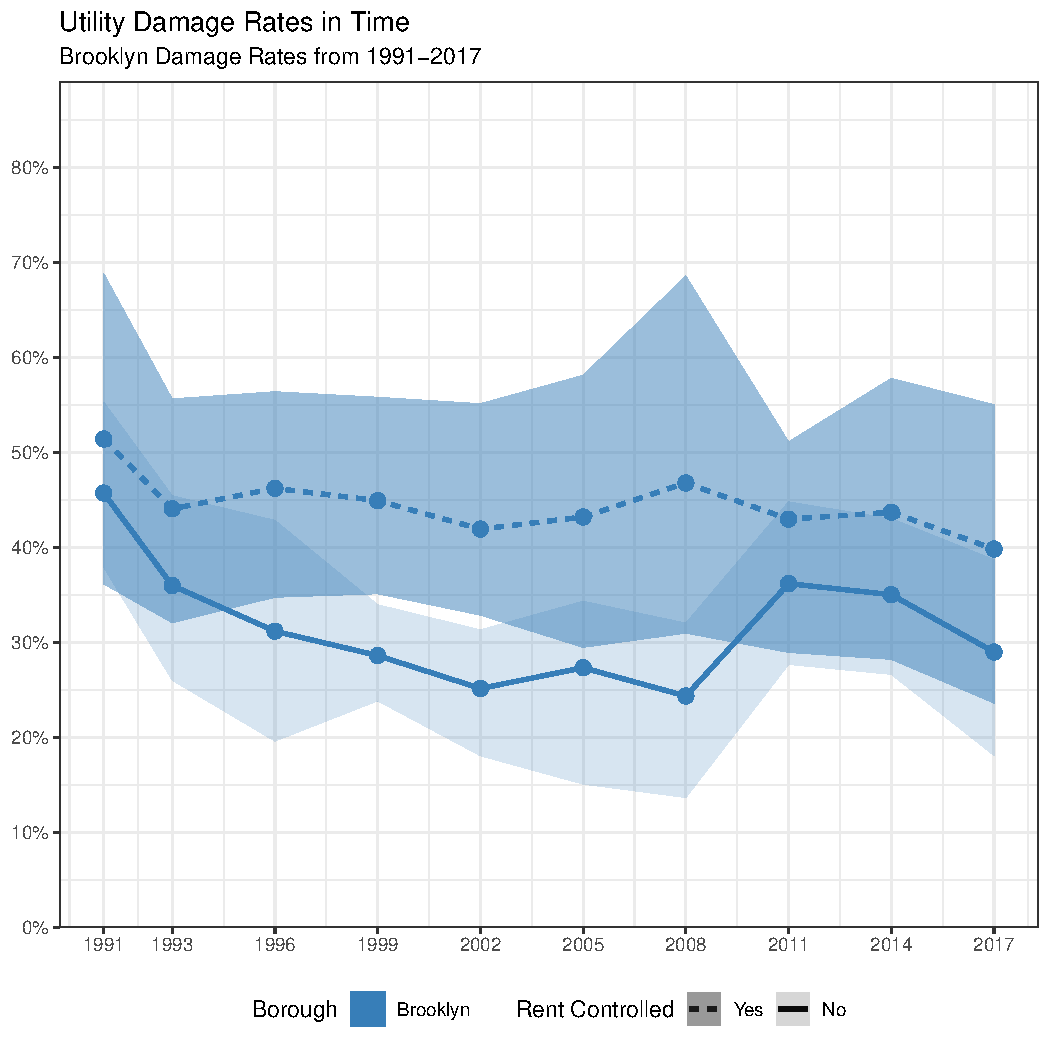
\includegraphics[width=\maxwidth]{figure/fig2-1} 

\end{knitrout}
\end{center}
\caption{Brooklyn Utility Damage Rates over Time Plot}
\label{fig:two}
\end{figure}
 
\section{Methods\label{methods}}
\subsection{Bayes Regularization}



During the aggregation process, we ran into a problem with some of the sub-borough level proportions. In some cases, there would only be a few homes to represent the rent controlled or non-rent controlled homes within a rent quartile for a sub-borough. So, if there are only a few houses and they all have or do not have a damage present, the estimated proportion for the whole sub-borough becomes 100\% or 0\%. This is clearly incorrect, so we must do some form of correction to the proportions to ensure the sub-boroughs proportions are being accurately represented. Through Bayes regularization using a Beta conjugate with shape parameters chosen from groupings that didn’t result in a 0\% or 100\%, we were able to ‘fix’ the proportions to ensure the groups with few houses to represent the entire group have accurate proportions we can use in the modeling stage. 

\[
\mathbf{p} = \frac{n}{n+\alpha+\beta}*\hat{p}+\frac{\alpha+\beta}{n+\alpha+\beta}*\frac{\alpha}{\alpha+\beta}
\]

\begin{figure}
\begin{center}
\begin{knitrout}
\definecolor{shadecolor}{rgb}{0.969, 0.969, 0.969}\color{fgcolor}
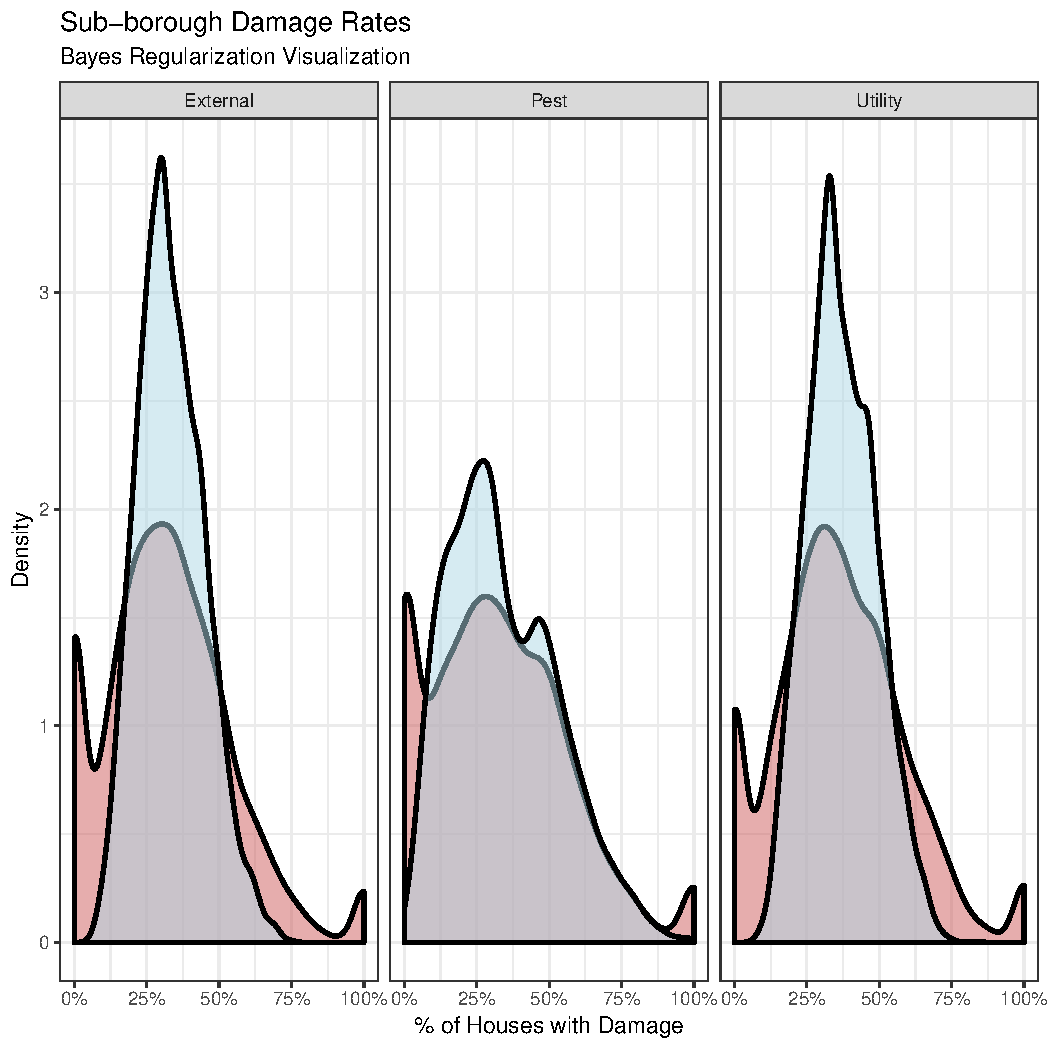
\includegraphics[width=\maxwidth]{figure/fig3-1} 

\end{knitrout}
\end{center}
\caption{Sub-borough damage rate distribution plots with bayes regularization}
\label{fig:three}
\end{figure}

\subsection{Model}
The model we decided to fit was a mulitple response multivaraite model that use the transformed log odds ratio of the damage proportions as a response and the year, rent quartile, rent control, borough, interaction of rent control and time, and interaction of rent control and rent quartile as predictor variables. The response is of the form:

\[
\mathbf{Y} = 
\left[
\begin{matrix} 
log\left(\frac{External}{1-External}\right)\\
log\left(\frac{Utility}{1-Utility}\right) \\
log\left(\frac{Pest}{1-Pest}\right) 
\end{matrix}
\right]
\]

The predictors variables we used to model the response are as follows. Rent Control (RC) has a value 1 if home is under rent control policy, 0 if otherwise. Ith Rent Quartile (Qi) is 1 if home falls into the ith rent quartile, 0 if otherwise and if all are 0 the home is in the 1st rent quartile. Year (T) has a value of 1990 subtracted from the year of the observation. Brooklyn has a value 1 if home is in Brooklyn, 0 if otherwise. Manhattan has a value 1 if home is in Manhattan, 0 if otherwise. Queens has a value 1 if home is in Queens, 0 if otherwise. StatenIsland has a value 1 if home is in StatenIsland, 0 if otherwise. If all borough variables have a value of 0, then the home is in the Bronx.

\begin{align*}
\mathbf{Y} = &\boldsymbol{\beta_0}+\\
&\boldsymbol{\beta_1}*T+\\
&\boldsymbol{\beta_2}*Q2+
\boldsymbol{\beta_3}*Q3+
\boldsymbol{\beta_4}*Q4+\\
&\boldsymbol{\beta_5}*RC+\\
&\boldsymbol{\beta_6}*Brooklyn+
\boldsymbol{\beta_7}*Manhattan+
\boldsymbol{\beta_8}*Queens+
\boldsymbol{\beta_9}*StatenIsland+\\
&\boldsymbol{\beta_{10}}*RC*T+\\
&\boldsymbol{\beta_{11}}*RC*Q2+
\boldsymbol{\beta_{12}}*RC*Q3+
\boldsymbol{\beta_{13}}*RC*Q4
\end{align*}

\section{Results\label{results}}
The fitted model coefficients for each response can be seen below, allowing for interpretation of model coefficients.

\begin{knitrout}
\definecolor{shadecolor}{rgb}{0.969, 0.969, 0.969}\color{fgcolor}\begin{kframe}
\begin{verbatim}
## [1] "this is where i will put the plot I am working on"
## [1] "that we discussed in our last meeting"
##                        logodds.external1 logodds.utility1 logodds.pest1
## (Intercept)                 -0.493533756     -0.292947930  -0.759181146
## RentControl1                 0.271756303      0.299395199   0.227396648
## Quartile2                   -0.058595041     -0.114198450  -0.167299474
## Quartile3                   -0.119033412     -0.184967863  -0.264667815
## Quartile4                   -0.223564559     -0.202220660  -0.365791108
## year                        -0.006505077     -0.007556319   0.024499182
## borough2                    -0.177031792     -0.236393255  -0.265643194
## borough3                    -0.036493198     -0.153671905  -0.418226412
## borough4                    -0.452288602     -0.436284258  -0.720474528
## borough5                    -0.442607786     -0.487297728  -1.019234214
## RentControl1:Quartile2       0.038081660      0.129384122   0.118470653
## RentControl1:Quartile3       0.045455023      0.181220262   0.271324737
## RentControl1:Quartile4       0.115675655      0.165021394   0.356153120
## RentControl1:year           -0.001466792     -0.001915774   0.006100295
\end{verbatim}
\end{kframe}
\end{knitrout}


This allows for a closer look at the modeled relationship between rent control and the three damages. The rent control effect coefficient confidence interval for the external damage is (0.1963, 0.3472), for utility damage is (0.2269, 0.3719), for pest present (0.0917, 0.3631). All three of these are positive, significant predictors which indicates that homes under rent control are correlated with larger log odds of all three damage rates, indicating that home under rent control are correlated with higher damage rates in all three cases.

A few other interesting modeled effects can be seen by looking at the non-zero coefficients. It appears that the aforementioned higher damage rates for rent controlled homes is larger for homes with higher monthly rent values. Perhaps indicating that rent controlled homes that charge higher monlthy rent are correlated with a larger gap in the damage rates between rent controlled and non rent controlled homes. Houses from Queens and Staten Island have lower damager rates than houses from the Bronx, Brooklyn, and Manhattan, indicating there is some relationship between borough a house resides in and the damage rates for all three categories. The proportion of homes with pests present has risen over time, perhaps due to survey changes, or better reporting of pests. The proportion of homes with external and utility damage has fallen over time, perhaps indicating a that damage rates across all of New York have been decreasing over time.

\section{Conclusions\label{conclusions}}
In conclusion, through this modeling process we were able measure the relationship between the set of predictor variables and the three damage rates. This resulted in the isolation of a significant correlations between rent control status of a home and higher damage rates in all three measures of damage.  While damage rates do tend to be decreasing over time, rent control has appears to be having a negative impact on housing quality. Perhaps an explanation for this trend could be that landlords are less incentivized to improve/maintain a unit when the current occupants have a monthly rent cost that is fixed so there isn’t an avenue to increase income from the property. The purpose of rent control is not just to control the costs of living and create affordable housing, the aim is to create affordable quality housing. In the current form, when controlling for other factors, a house under rent control is more likely to have damages which means rent control is not fulfilling the quality housing portion of its goal. This could indicate that rent control policy could use a change in methodology or implementation because while the current methods are creating affordable housing, the housing is not of the same quality of a similar house that is not under rent control policy. Identifying this trend creates the opportunity to change current methods to see if you can change the current relationship between rent control and housing damages.


\end{document}
